\documentclass[preprint]{aastex}
\usepackage{amsmath, amsfonts, amssymb}
\usepackage{fullpage}
\usepackage[colorlinks,urlcolor=blue,citecolor=blue,linkcolor=blue]{hyperref}

\slugcomment{Draft: \today}
\shorttitle{ATA Beam Squint}
\shortauthors{Burns et al.}

\begin{document}
\title{Characterizing Beam Size and Squint at the ATA}
\author{Keaton J. Burns, Peter K. G. Williams, \and Geoffrey C. Bower}

\begin{abstract}
We present a study of primary beam size and squint in the antennas and
feeds at the Allen Telescope Array, based on weekly calibrator
observations in small mosaicked patterns. A relational database of
beam parameters was created, which reduces the results of an upgraded
and automated analysis pipeline.  A Python visualization tool was
developed to efficiently interface with the squint database and search
for correlations in this large dataset.  We find that \ldots
\end{abstract}


%%%%%
\section{Introduction}\label{s.intro}
Yadda yadda Allen Telescope Array \citep[ATA;][]{Welch2009}.

ATA telescope calibration is accomplished through observing known
radio point sources to determine the system temperature, pointing
centers, and beam shape for each antenna.  One parameter of interest
from these observations is telescope squint, which we define as the
offset of the Y polarization pointing center from the X polarization
pointing center, in azimuth and altitude.  Knowledge of each
telescope's squint is useful for assessing the reliability of data
from each polarization based on each telescope's pointing model
(e.g., for large-squint telescopes, pointing models based on X
polarization pointing centers yield suboptimal Y polarization
data). Studying telescope squint also provides insights into the
strengths and limitations of the offset-Gregorian dish and
log-periodic feed designs used at the ATA, and may be useful for
directing future telescope development.  Our aims in this project
included isolating the cause of the squint to the feed or dish,
studying the effects of feed upgrades on the squint, and assessing the
stability of a telescope's squint with changes in frequency and time.


%%%%%
\section{Observations}\label{s.observations}

Measurements of primary beam (PB) shape and squint were obtained by
weekly observations of bright, compact sources from 2009~Oct~17 to
2011~Apr~06. The core observing pattern in each session consisted of
an observation pointed directly at the source followed by a small
mosaic of pointings offset from the source by an angle comparable to
half of the nominal PB full-width at half maximum (FWHM). Each
pointing lasted for 60--90 seconds, with a typical pattern taking
about 20 minutes to observe (including overheads). In the significant
majority of cases, the small mosaic consisted of six additional
pointings arranged in a equilateral hexagon around the central
source. Two points of the hexagon were on a line of constant
declination matching that of the source and the distance between
pointings was exactly half of the nominal PB FWHM. Other pointing
patterns, such as crosses or nested hexagons, and other offset sizes,
such as one quarter of the FWHM, were occasionally used.  The sources
3C\,48, 3C\,138, 3C\,147, and 3C\,286 were used as targets, with the
selection depending on visibility and higher-elevation sources being
preferred.

At the time of the observations, the ATA had two independently-tunable
correlators able to access any central frequency within the facility's
overall accessible band, 0.5--11~GHz. Each observing session included
several cycles of observing patterns with the correlators tuned to
several pairs of frequencies. Most observations were made with paired
central frequencies of 0.7 \& 1.43, 2.01 \& 3.14, or 5.00 \&
7.60~GHz. Each correlator had a bandwidth of 104~MHz divided into 1024
spectral channels.

Because the position of the focal point of the ATA optical path is
wavelength-dependent, each ATA feed is mounted on a piston that allows
repositioning of the feed for optimal match to one of the observing
frequencies. Feed performance degrades for frequencies above the
commanded ``focus frequency'' while it remains fairly good for those
below it \citep{Harp2011}. In these observations the focus was always
set to be optimal for the higher of each pair of observing
frequencies.

\section{Data Reduction}\label{s.reduction}

After each observing session the data were reduced with an automated
pipeline. The observation of the central pointing of each observing
pattern was automatically flagged for radiofrequency interference
(RFI) and gain- and bandpass-calibrated using the COMPASS system
developed for the ATA \citep{Keating2010}. The rest of the scans were
likewise automatically flagged and had the calibrations from the
central pointing applied. Some scans were discarded due to excessive
RFI or problems in digital hardware; if the central pointing was
discarded, the whole pointing pattern was as well.

Each ATA feed is sensitive to two orthogonal linear polarizations, $X$
(horizontal relative to ground) and $Y$ (vertical). Only parallel-hand
correlations were processed, so that the $X$ and $Y$ correlations were
effectively reduced independently. We refer to the signal originating
from a particular polarization on a particular antenna as coming from
a certain ``antpol''. In some antennas, only one antpol was
correlated.

After initial calibrations were applied, the MIRIAD \citep{Sault1995}
task \textsf{selfcal} was used on each side pointing to derive complex
correction gains for each antpol. An additional program was written to
determine uncertainties in the solved-for gains, which are not
reported by \textsf{selfcal}. Because the received flux in all fields
is dominated by the central calibrator source, these gains can be
interpreted as the inverse of the complex PB response associated with
each antpol in the direction of the calibrator, where the response
towards pointing center is unity. These gains may vary between antpols
on the same antenna due to differences in the spatial response of the
$X$ and $Y$ receptors or polarization leakage in the overall optical
path.

Two-dimensional (2D) Gaussian profiles in azimuth-elevation (az-el)
space were fit to the measurements of each antpol in each pointing
pattern. Because the pointing patterns on the sky were aligned to the
equatorial coordinate system, the az-el offsets probed varied as a
function of parallactic angle and did not trace out precisely uniform
figures. Each Gaussian fit had five free parameters: offsets in
azimuth and elevation from pointing center; characteristic widths in
azimuth and elevation; and an overall amplitude scaling. The fits
resulted in measurements of these parameters, their formal
uncertainties, and a reduced $\chi^2$ value for the overall
result. Other data products of the pipeline included the relative
complex gain values, post-hoc measurements of the system equivalent
flux density (SEFD) for each antpol, and images of the central
pointings.

\subsection{Squint Database}\label{ss.database}
The Gaussian fit parameters from all runs were imported into a
relational database for analysis. For those antennas for which data
from both polarizations were available, squint vectors were calculated
as defined in \S\ref{s.intro}.

A query program use the Structured Query Language (SQL) to retrieve
and plot data with arbitrary filtering and transformation of the
underlying values. Derived data such as squint magnitudes and angles,
and their respective uncertainties, are computed during retrieval.

\subsection{Outlier Removal}\label{ss.outliers}
A mechanism was implemented to exclude bad data from downstream
analyses.  To remove bad observations, and particularly poor reduction
fits, observations with frequency-normalized squint or width
components in the top percentile, or uncertainties above the
98$^\textrm{th}$ percentile, were flagged as outliers.  Observations
above the 98$^\textrm{th}$ percentile of SEFD and the 90$^\textrm{th}$
percentile of the Gaussian fit $\chi^2$ value were also flagged.  The
$\chi^2$ cutoff is at a significantly lower percentile, as it is a
direct indicator of the convergence of the Gaussian fits, and there
were a significant number of outliers in this parameter, as shown in
Fig.~\ref{fig.dist_sumchisq}.

Nearly all observations at 700 MHz, the lowest observed frequency,
were flagged under these conditions, so the remaining observations
were also excluded.  Additionally, data at 3140 MHz revealed a strong
beam size and shape dependence on the observed source, seemingly
caused by source confusion, prompting us to discard all but the 3c48
observations (see Fig.~\ref{fig.source_confusion}). After removal of
these data, 1309 observations remained.

\begin{figure}[htb]
\begin{center}
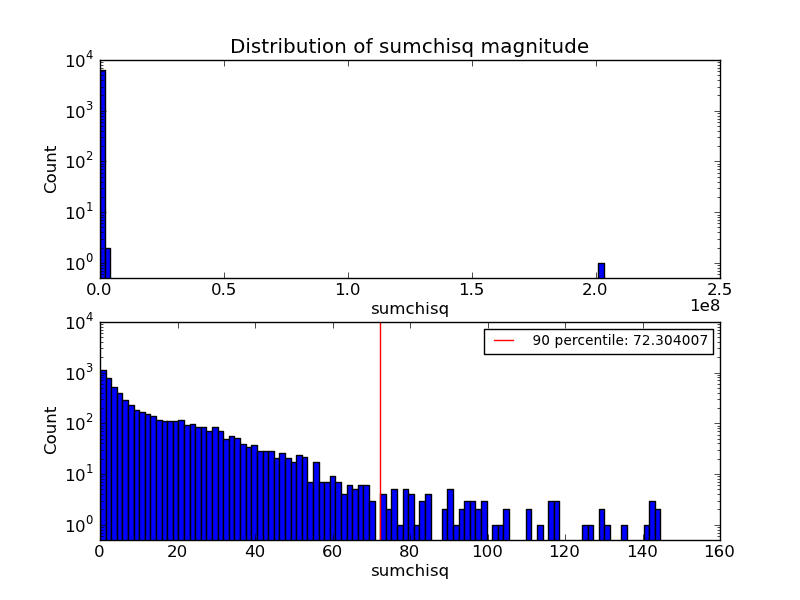
\includegraphics[width=0.7\textwidth]{images/dist_sumchisq}
\caption{Top: Distribution of $\chi^2$ values for 2D Gaussian primary
  beam fits across all observations.  Bottom: Zoom-in at outlier
  cutoff at the 90$\textrm{th}$ percentile. \label{fig.dist_sumchisq}}
\end{center}
\end{figure}

\begin{figure}[htb]
\begin{center}
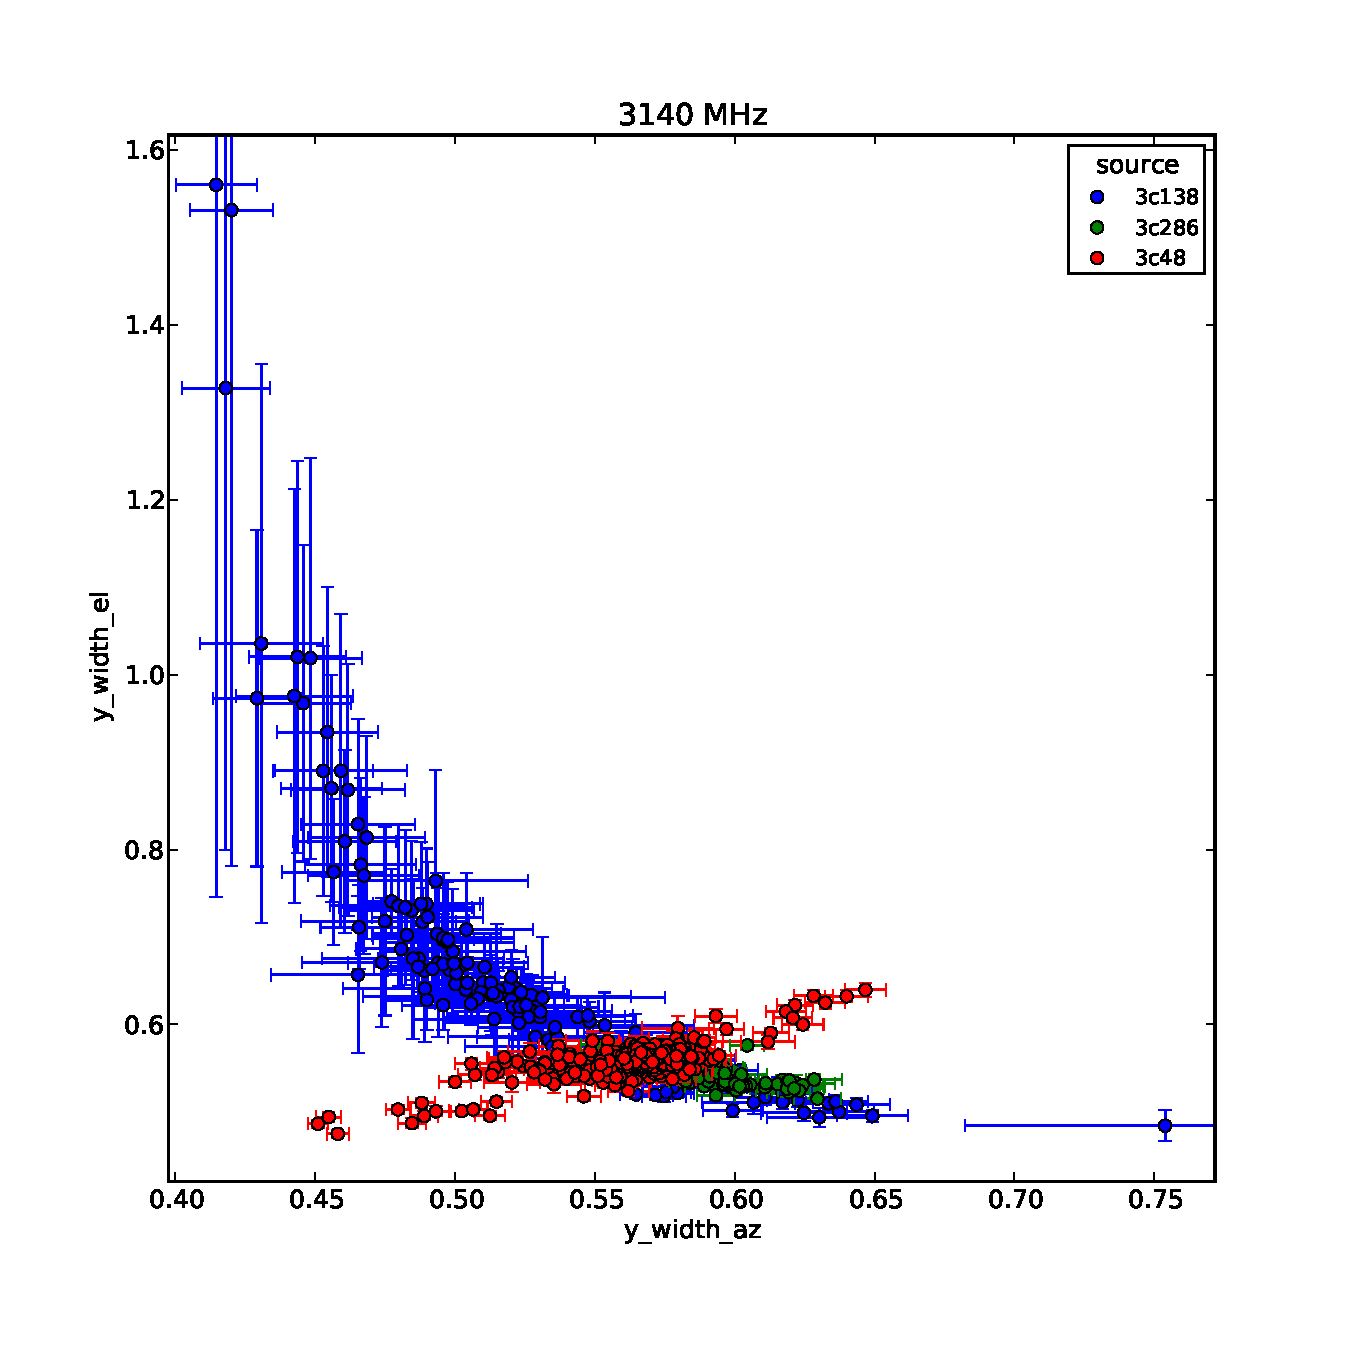
\includegraphics[width=0.8\textwidth]{images/source_confusion}
\caption{Source confusion in 3140 MHz observations.  Source 3c48 used
  for analysis. \label{fig.source_confusion}}
\end{center}
\end{figure}


%%%%%
\section{Analysis and Results}\label{s.results}

\subsection{Primary Beam Size}\label{ss.beamsize}
Scatterplots depicting the PB shape (best-fit 2D Gaussian
elevation width vs azimuthal width) for the X and Y polarizations are
depicting in Figures~\ref{fig.x_widths} and \ref{fig.y_widths}
respectively, and Table \ref{tab.widths} gives the means and standard
deviations of these values.  We find general agreement with the
approximate results of \citet{Harp2011}, namely $\textrm{FWHM} \approx
3.5^{\circ} / f_\textrm{GHz}$.

\begin{table}[htb]
\begin{center}
\begin{tabular}{cccc}
Polarization & Direction & Mean [$^{\circ} / f_\textrm{GHz}$] & St. Dev \\
\hline
X & El & 3.663 & 0.245 \\
X & Az & 3.443 & 0.216 \\
Y & El & 3.568 & 0.331 \\
Y & Az & 3.568 & 0.303
\end{tabular}
\caption{Best-fit primary beam width averages \label{tab.widths}}
\end{center}
\end{table}

\begin{figure}[htb]
\begin{center}
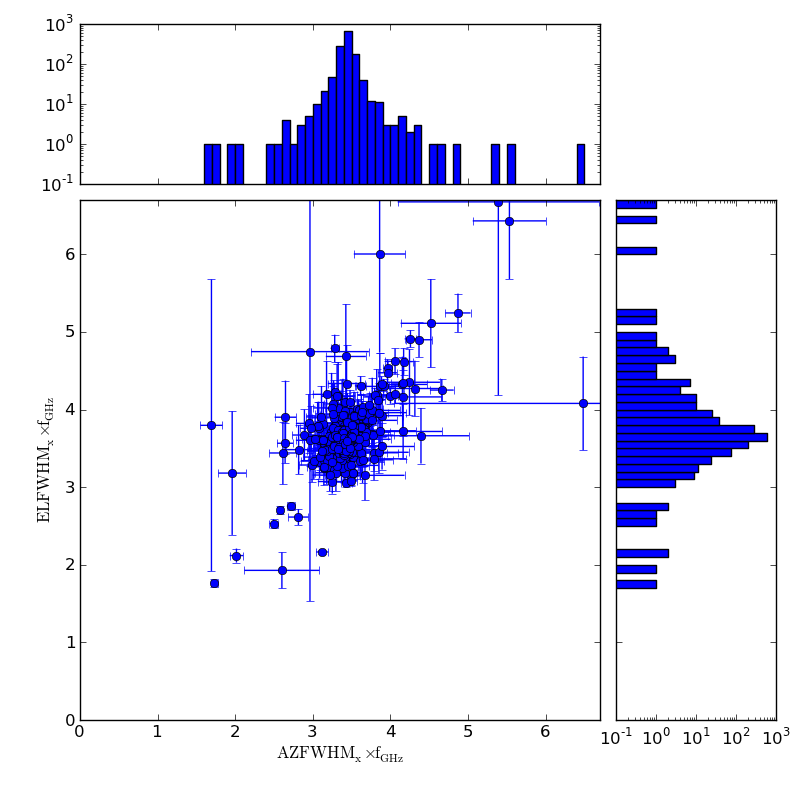
\includegraphics[width=0.8\textwidth]{images/x_widths}
\caption{X polarization primary beam widths. \label{fig.x_widths}}
\end{center}
\end{figure}

\begin{figure}[htb]
\begin{center}
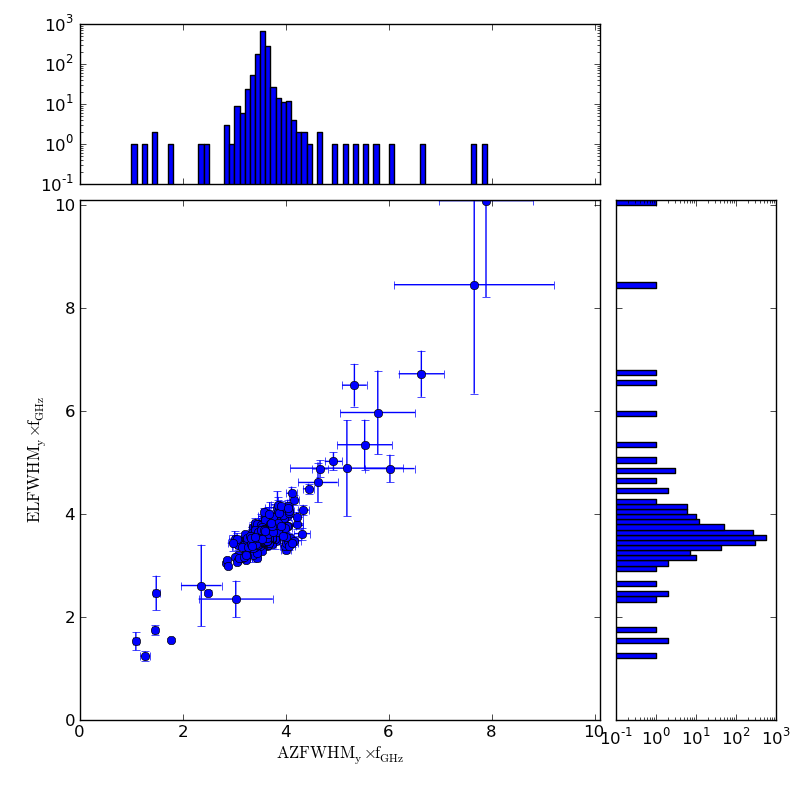
\includegraphics[width=0.8\textwidth]{images/y_widths}
\caption{Y polarization primary beam widths. \label{fig.y_widths}}
\end{center}
\end{figure}

\subsection{Squint: Temporal Variation}\label{ss.temporal}

\subsection{Squint: Feed vs. Antenna}\label{ss.antfeed}

\subsection{Squint: Effects of Feed Revisions}\label{ss.revisions}

\subsection{Squint: Frequency Dependence}\label{ss.freq}
To study the effects of frequency on squint, for each antfeed, we
performed a linear least-squares fit on the log of squint magnitude
and the log of frequency for each observing run.  The slope of this
fit represents the best fitting power-law index $\alpha$, assuming
$|\vec{S}| \propto f^\alpha$.  We then took the median power-law index
across all observing runs for each antfeed.

The best fitting linear slope was similarly computed for each antfeed
(fitting squint magnitude to frequency, assuming a power-law index of
1).  Histograms of these indices and slopes are displayed in figure
NEEDREF.  The same plots were generated with the data separated by
feed revision.  We notice substantial spread in the power-law indices,
mainly between 0 and -2.  We note that the data for for feed revision
3 show less spread (0 to -1) than the other revisions.

%%%%%
\section{Conclusions}\label{s.conclusions}
This is where we conclude.


%%%%%
\acknowledgments
Research with the ATA is supported by the Paul G. Allen Family
Foundation, the National Science Foundation, the US Naval Observatory,
and other public and private donors. This research has made use of
NASA's Astrophysics Data System.

Facilities: \facility{ATA}

\bibliographystyle{yahapj}
\bibliography{ATA.bib}

\end{document}
